\documentclass[11pt,letterpaper]{article}
\usepackage[lmargin=1in,rmargin=1in,tmargin=1in,bmargin=1in]{geometry}
\usepackage{../style/homework}
\usepackage{../style/commands}
\setbool{quotetype}{true} % True: Side; False: Under
\setbool{hideans}{false} % Student: True; Instructor: False

% -------------------
% Content
% -------------------
\begin{document}

\homework{6: Due 10/13}{Good rain knows the best time to fall.}{VIP, Squid Game}


% Problem 1
\problem{10} Consider the function $\ell(x)= 5x + 2$.

\begin{enumerate}[(a)]
\item What is the graph of the function $\ell(x)$.
\item Find two points on the graph of $\ell(x)$.
\item Is the point $(2, 5)$ on the graph of $\ell(x)$? Explain. 
\item Is the point $(-1, -3)$ on the graph of $\ell(x)$? Explain. 
\end{enumerate} \pspace

\sol

\begin{enumerate}[(a)]
\item Because the function $\ell(x)$ is of the form $mx + b$, $\ell(x)$ is a linear function. But then the graph of $\ell(x)$ is a line. 

\item To find points on $\ell(x)$, we choose $x$-values and find the corresponding $y$-values. If $x= 0$, then $\ell(0)= 5(0) + 2= 0 + 2= 2$. Therefore, $(0, 2)$ is a point on the graph of $\ell(x)$. If $x= 1$, then $\ell(1)= 5(1) + 2= 5 + 2= 7$. Therefore, $(1, 7)$ is also a point on the graph of $\ell(x)$. 

\item The point $(2, 5)$ has $x$-value $2$. Then if $(2, 5)$ is on the graph of $\ell(x)$, it must be that $\ell(2)= 5$. We check this. Observe $\ell(2)= 5(2) + 2= 10 + 2= 12 \neq 5$. Therefore, $(2, 5)$ is not on the graph of $\ell(x)$. 

\item The point $(-1, -3)$ has $x$-value $-1$. Then if $(-1, -3)$ is on the graph of $\ell(x)$, it must be that $\ell(-1)= -3$. We check this. Observe $\ell(-1)= 5(-1) + 2= -5 + 2= -3$. Therefore, $(-1, -3)$ is on the graph of $\ell(x)$. 
\end{enumerate}





\newpage





% Problem 2
\problem{10} Do the points $(5, 2)$, $(1, -1)$, and $(-3, 4)$ lie along a line? Explain. \pspace

\sol The slope of a line is constant. Therefore, if all the points lie along a line, the slope calculated through each of these points must be the same. Observe\dots
	\[
	\begin{aligned}
	m_1&= \dfrac{2 - (-1)}{5 - 1}= \dfrac{2 + 1}{5 - 1}= \dfrac{3}{4} \\[0.3cm]
	m_2&= \dfrac{-1 - 4}{1 - (-3)}= \dfrac{-1 - 4}{1 + 3}= \dfrac{-5}{4}
	\end{aligned}
	\]
Because the slopes are not the same, these points do not all lie along a line. 





\newpage





% Problem 3
\problem{10} Consider the line given by the function $\ell(x)= 1 - 3x$.

\begin{enumerate}[(a)]
\item Write this line in the form $Ax + By= C$ for some $A, B, C$. 
\item What is the slope of this line?
\item Find the $y$-intercept of the line.
\item Find the $x$-intercept of the line. 
\end{enumerate} \pspace

\sol
\begin{enumerate}[(a)]
\item We replace $\ell(x)$ with $y$. Then we have $y= 1 - 3x$. Then we have $3x + y= 1$. But then this is a line of the form $Ax + By= C$, where $A= 3$, $B= 1$, and $C= 1$. 

\item Examining $\ell(x)= 1 - 3x$, we see that the slope of this line is $-3$. 

\item The $y$-intercept is where the curve passes through the $y$-axis. This is where $x= 0$. But we have $\ell(0)= 1 - 3(0)= 1 - 0= 1$. Therefore, the $y$-intercept is the point $(0, 1)$. 

\item The $x$-intercept is where the curve passes through the $x$-axis. This is where $y= 0$, i.e. $\ell(x)= 0$. But then
	\[
	\begin{aligned}
	\ell(x)&= 0 \\
	1 - 3x&= 0 \\
	3x&= 1 \\
	x&= \dfrac{1}{3}
	\end{aligned}
	\]
Therefore, the $x$-intercept is the point $(\frac{1}{3}, 0)$. 
\end{enumerate}





\newpage





% Problem 4
\problem{10} Are the following lines parallel, perpendicular, or neither? Explain.
	\[
	\begin{aligned}
	y&= 2x - 5 \\
	2y&= 4x - 8
	\end{aligned}
	\] \pspace

\sol We want each line in the form $y= mx + b$. The first line is already in this form. For the second line, we divide both sides by 2 to obtain $y= 2x - 4$. The slope of the first line is $m= 2$. The slope of the second line is $m= 2$. Because the lines have equal slope, the lines are parallel. 





\newpage





% Problem 5
\problem{10} Are the following lines parallel, perpendicular, or neither? Explain.
	\[
	\begin{aligned}
	y&= \frac{2}{3}\,x + 7 \\
	2x &+ 3y= 5
	\end{aligned}
	\] \pspace

\sol We want each line in the form $y= mx + b$. The first line is already in this form. For the second line, we solve for $y$. We have $y= \frac{5}{3} - \frac{2}{3}x$. The slope of the first line is $m= \frac{2}{3}$. The slope of the second line is $m= -\frac{2}{3}$. Perpendicular lines have negative reciprocal slopes. The negative reciprocal of $\frac{2}{3}$ is $-\frac{3}{2}$. Because the slopes are not negative reciprocals, the lines are not perpendicular. 





\newpage





% Problem 6
\problem{10} Find the equation of the line plotted below.
	\[
	\fbox{
	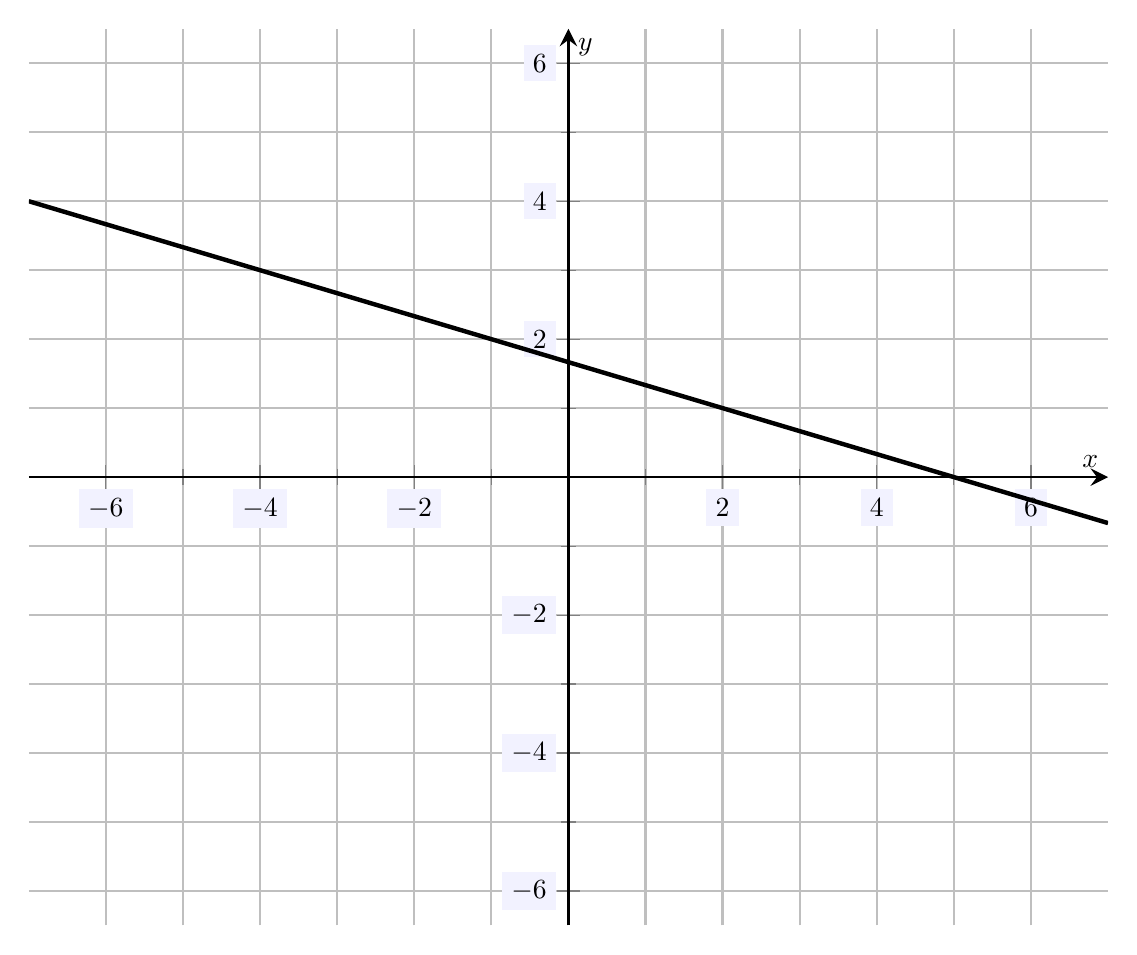
\begin{tikzpicture}[scale=2,every node/.style={scale=0.5}]
	\begin{axis}[
	grid=both,
	axis lines=middle,
	ticklabel style={fill=blue!5!white},
	xmin= -7, xmax=7,
	ymin= -6.5, ymax=6.5,
	xtick={-6,-4,-2,0,2,4,6},
	ytick={-6,-4,-2,0,2,4,6},
	minor tick = {-5,-3,...,5},
	xlabel=\(x\),ylabel=\(y\),
	]
	\addplot[thick, domain= -7:7] {-1/3*x + 5/3};
	\end{axis}
	\end{tikzpicture}
	}
	\] \pspace

\sol We see that the line passes through the points $(-4, 3), (2, 1), (5, 0)$. We compute the slope of the line using two of the points:
	\[
	m= \dfrac{0 - 1}{5 - 2}= \dfrac{-1}{3}= -\dfrac{1}{3}
	\]
Now we use the fact that the line must be of the form $y= mx + b$ (because the line is not vertical). Using the point $(5, 0)$, i.e. $x= 5$ and $y= 0$, we find
	\[
	\begin{aligned}
	y&= mx + b \\
	y&= -\frac{1}{3}x + b \\
	0&= -\frac{1}{3} \cdot 5 + b \\
	0&= -\frac{5}{3} + b \\
	b&= -\dfrac{5}{3}
	\end{aligned}
	\]
Therefore, the equation of the line is $y= -\dfrac{1}{3}\,x - \dfrac{5}{3}= \dfrac{-x - 5}{3}= - \dfrac{x + 5}{3}$.





\newpage





% Problem 7
\problem{10} Solve the following equation for $y$:
	\[
	5x - 3y= 12
	\] \pspace

\sol We have\dots
	\[
	\begin{aligned}
	5x - 3y&= 12 \\
	-3y&= 12 - 5x \\
	y&= \dfrac{12}{-3} - \dfrac{5}{-3}\,x \\
	y&= -4 + \dfrac{5}{3}\,x \\
	y&= \dfrac{5}{3}\,x - 4
	\end{aligned}
	\]


%\printpoints
\end{document}